\documentclass{beamer}

%! TeX program = pdflatexpre

\usepackage{beamer_digiPH}
\usepackage[bahasai]{babel}


%----------------------------------------------------------------------------------------
%	FONTS
%----------------------------------------------------------------------------------------

\usepackage[utf8]{inputenc} % Required for inputting international characters
\usepackage[T1]{fontenc} % Use 8-bit encoding

\usepackage[protrusion=true, expansion=true]{microtype} % Better typography

\linespread{1.05} % Increase line spacing slightly; Palatino benefits from a slight increase by default

%----------------------------------------------------------------------------------------
%	PACKAGES AND OTHER DOCUMENT CONFIGURATIONS
%----------------------------------------------------------------------------------------

\usepackage{comment}
\usepackage{lipsum}

\usepackage{graphicx}
\graphicspath{{figures/}{../figures/}{../logos}}

%Position figure in beamer using textblock*
\usepackage[absolute,overlay]{textpos}
%\usepackage[texcoord,grid,gridunit=mm,gridcolor=red!10,subgridcolor=green!10]{eso-pic} %showgrid

\usepackage{setspace}
\usepackage{subfiles}

\usepackage{booktabs}
\usepackage{csquotes}
\usepackage{xcolor}


% Turn off the floating in article mode
\usepackage{float}

\usepackage{xspace}
\newcommand{\zB}{z.\,B.\xspace}
\usepackage{xfrac}
\UseCollection{xfrac}{plainmath}

% Config Slide Notes
\usepackage{pgfpages}

\setbeamercovered{transparent}
\setbeamertemplate{note page}{\pagecolor{yellow!5}\insertnote}\usepackage{palatino}


\usepackage{multirow}
\usepackage{booktabs}
\usepackage{tabularx}
\usepackage{array} %Mostly formatting columns and spacing
\newcolumntype{P}[1]{>{\centering\arraybackslash}p{#1}} %centering elemen in table
\newcommand{\tabitem}{~\llap{\textbullet}} % fake bullet itemize in table cell
\newcommand{\tabitems}{~~\llap{\textbullet}~~}

% Itemize
\usepackage{enumitem} %3 lines after this resolve bullet disappear and adjust spacing
\setitemize{label=\usebeamerfont*{itemize item}%
	\usebeamercolor[fg]{itemize item}
	\usebeamertemplate{itemize item},noitemsep,topsep=0pt,parsep=0pt,partopsep=0pt}


%----------------------------------------------------------------------------------------
%           SOMETHING ABOUT LABELING
%----------------------------------------------------------------------------------------


\makeatletter
\newenvironment{labeling}[2][]{%
	\def\sc@septext{#1}%
	\list{}{\settowidth{\labelwidth}{{%
					#2%
					\sc@septext%
				}}%
		\leftmargin\labelwidth \advance\leftmargin by \labelsep
		\let\makelabel\labelinglabel
	}%
}{%
	\endlist
}
\newcommand\labelinglabel[1]{%
	#1\hfil
	\sc@septext%
}
\makeatother

%----------------------------------------------------------------------------------------
%           New Environment/cmd
%----------------------------------------------------------------------------------------
%new block environemtn
\newenvironment{blockcolor}
{\begin{alertblock}
		}
		{

		\centering
		\includegraphics[width=2cm,trim={0cm 10cm 0cm 9cm}, clip]{figures/batik.png}
	\end{alertblock}
}

% Creating centering notes
\newcommand{\notes}[1]{\note{\vfill
		%    \begin{center}
		{#1}
		%    \end{center}
		\vfill
	}}

\newcommand{\boxes}[3]{\begin{tpblock}{#1}{#2} #3 \end{tpblock}}

%----------------------------------------------------------------------------------------
%           BLOCK
%----------------------------------------------------------------------------------------
\usepackage[most]{tcolorbox}
\newtcolorbox{tpblock}[3][]
{%
	code={%
			\usebeamercolor{block title}
			\colorlet{titlebg}{#2}
			\colorlet{titlefg}{#3}
			\usebeamercolor{block body alerted}
			\colorlet{bodybg}{#2}
			\colorlet{bodyfg}{#3}
		},
	enhanced,
	boxsep=0.25ex,
	arc=1.25ex,
	opacityframe=.2,
	opacityback=.2,
	colbacktitle=titlebg,
	coltitle=titlefg,
	colback=bodybg,
	colupper=bodyfg,
	boxrule=0pt,
	#1
}

%----------------------------------------------------------------------------------------
%           TIKZ PLOT CONFIGURATION
%----------------------------------------------------------------------------------------

% Paket zum Erstellen von Plots mit TikZ
\usepackage{pgfplots}
% immer die neueste Version benutzen
\pgfplotsset{compat=newest}
% Verbindung von Linien durch eine schräge Kante
\pgfplotsset{every axis/.append style={line join=bevel}}
% Formatvorlage für Präsentationen
\mode<beamer>{
	\pgfplotsset{
		beamer/.style={
				width=0.8\textwidth,
				height=0.45\textwidth,
				legend style={font=\scriptsize},
				tick label style={font=\footnotesize},
				label style={font=\small},
				max space between ticks=28,
			}
	}
}
\mode<handout>{
	\pgfplotsset{
		beamer/.style={
				width=0.8\textwidth,
				height=0.45\textwidth,
				legend style={font=\scriptsize},
				tick label style={font=\footnotesize},
				label style={font=\small},
				max space between ticks=25,
			}
	}
}
\mode<article>{
	\pgfplotsset{
		beamer/.style={
				width=0.8\textwidth,
				height=0.45\textwidth,
				max space between ticks=35,
			}
	}
}
% neue Größenvorlage für zwei Plots nebeneinander anlegen
\pgfplotsset{
	scriptsize/.style={
			width=0.34\textwidth,
			height=0.1768\textwidth,
			legend style={font=\scriptsize},
			tick label style={font=\scriptsize},
			label style={font=\footnotesize},
			title style={font=\footnotesize},
			every axis title shift=0pt,
			max space between ticks=25,
			every mark/.append style={mark size=7},
			major tick length=0.1cm,
			minor tick length=0.066cm,
		}
}
\pgfplotsset{
	small/.style={
			width=6.5cm,
			height=,
			tick label style={font=\footnotesize},
			label style={font=\small},
			legend style={font=\footnotesize},
			max space between ticks=30,
		}
}
% Legendeneintrage standardmäßig links ausrichten
\pgfplotsset{legend cell align=left}
% Hauptgitternetz zeichnen
\pgfplotsset{xmajorgrids}
\pgfplotsset{ymajorgrids}
% Anzahl der kleinen Teilstriche zwischen zwei großen Teilstrichen
%\pgfplotsset{minor x tick num={3}}
%\pgfplotsset{minor y tick num={3}}
% feines Gitternetz zeichnen
%\pgfplotsset{xminorgrids}
%\pgfplotsset{yminorgrids}
% nur nach den Achsen skalieren
\pgfplotsset{scale only axis}
% Farben wie in MATLAB definieren
\definecolor{matlab1}{rgb}{0,0,1}
\definecolor{matlab2}{rgb}{0,0.5,0}
\definecolor{matlab3}{rgb}{1,0,0}
\definecolor{matlab4}{rgb}{0,0.75,0.75}
\definecolor{matlab5}{rgb}{0.75,0,0.75}
\definecolor{matlab6}{rgb}{0.75,0.75,0}
\definecolor{matlab7}{rgb}{0.25,0.25,0.25}
% Farbreihenfolge wie in MATLAB definieren
\pgfplotscreateplotcyclelist{matlab}{
	{matlab1,solid},
	{matlab2,dashed},
	{matlab3,dashdotted},
	{matlab4,dotted},
	{matlab5,densely dashed},
	{matlab6,densely dashdotted},
	{matlab7,densely dotted}% dies unterdrückt einen Fehler
}
% Farbreihenfolge wie in MATLAB benutzen
\pgfplotsset{cycle list name=matlab}
% Farbreihenfolge von pgfplots benutzen
%\pgfplotsset{cycle list name=color list}
% nur Graustufen benutzen
%\pgfplotsset{cycle list name=linestyles}
% Strichstärke auf 1pt festlegen
\pgfplotsset{every axis plot/.append style={line width=1pt}}
% für deutsche Dokumente ein Komma benutzen
\addto\extrasngerman{\pgfplotsset{/pgf/number format/.cd,set decimal separator={{{,}}}}}
% ein halbes Leerzeichen als Tausendertrennzeichen benutzen
%\pgfplotsset{/pgf/number format/.cd,1000 sep={\,}}
% kein Tausendertrennzeichen verwenden
\pgfplotsset{/pgf/number format/.cd,1000 sep={}}
% Zahlen kleiner als 0.1 auch im fixed-Format ausgeben
\pgfplotsset{/pgf/number format/.cd,std=-2}
% neue Positionen für Legenden anlegen
\pgfplotsset{/pgfplots/legend pos/north/.style={/pgfplots/legend style={at={(0.50,0.97)},anchor=north}}}
\pgfplotsset{/pgfplots/legend pos/south/.style={/pgfplots/legend style={at={(0.50,0.03)},anchor=south}}}
\pgfplotsset{/pgfplots/legend pos/east/.style={/pgfplots/legend style={at={(0.97,0.50)},anchor=east}}}
\pgfplotsset{/pgfplots/legend pos/west/.style={/pgfplots/legend style={at={(0.03,0.50)},anchor=west}}}
\pgfplotsset{/pgfplots/legend pos/outer north/.style={/pgfplots/legend style={at={(0.50,1.03)},anchor=south}}}

% Paket für SI-Einheiten
\usepackage[binary-units]{siunitx}
% Brüche aktivieren
\sisetup{per-mode=fraction}
% Dezimaltrennzeichen abhängig von der Sprache
\addto\extrasngerman{\sisetup{output-decimal-marker={,}}}
\addto\extrasenglish{\sisetup{output-decimal-marker={.}}}
% Trennzeichen für Bereiche
\addto\extrasngerman{\sisetup{range-phrase={ bis~}}}
\addto\extrasenglish{\sisetup{range-phrase={ to~}}}


% Bibliography
\usepackage[round]{natbib}
\setcitestyle{open={(},close={)}}

% How to remove some pages from the navigation bullets in Beamer?
% siehe: https://tex.stackexchange.com/questions/37127/how-to-remove-some-pages-from-the-navigation-bullets-in-beamer
\makeatletter
\let\beamer@writeslidentry@miniframeson=\beamer@writeslidentry
\def\beamer@writeslidentry@miniframesoff{%
	\expandafter\beamer@ifempty\expandafter{\beamer@framestartpage}{}% does not happen normally
	{%else
		% removed \addtocontents commands
		\clearpage\beamer@notesactions%
	}
}
\newcommand*{\miniframeson}{\let\beamer@writeslidentry=\beamer@writeslidentry@miniframeson}
\newcommand*{\miniframesoff}{\let\beamer@writeslidentry=\beamer@writeslidentry@miniframesoff}
\makeatother


\setbeameroption{hide notes} % Only slides
%\setbeameroption{show only notes} % Only notes
%\setbeameroption{show notes on second screen=right} % Both

\usepackage{beamer_digiPH}
\usepackage{comment}
\usepackage{lipsum}

\title{\#Lorem Ipsum}
\author{Muhammad Uliah Shafar}
\institute[Lehrstuhl]{
	Name des Lehrstuhls \\
	Name des Instituts/Fachbereichs \\
	Name der Universität, Ort
}
\mode<presentation>{\keywords{Schlüsselwörter durch Komma getrennt}}
\date[09.04.2018]{Datum der Präsentation, \zB 9. April 2018}

\begin{document}

\begin{withoutheadline}
%\begin{frame}
%	% Schriftgröße verkleinern
%	\small
%	% Absatzabstand einstellen
%	\setlength{\parskip}{0.75\baselineskip}
%
%	Dies ist die eLectures-Präsentationsvorlage der Virtuellen PH.
%
%	Die kommenden Folien in \LaTeX\ können und \textbf{\emph{sollen} Sie nach Wunsch adaptieren}, wir bitten Sie aber, sich alle genau anzusehen und durchzulesen! Denn:
%
%	Auf jeder Folie finden Sie Anregungen, Hilfestellungen und Hinweise, sowohl für die inhaltlich-didaktische Vorbereitung als auch die Präsentation online. Zumindest die vorhergehende Titelfolie sollte bitte auf jeden Fall in dieser Form Verwendung finden (Wiedererkennungswert!)
%
%	Bitte senden Sie Ihre überarbeitete PDF-Datei \textbf{vor dem gemeinsamen Testtermin} direkt an Ihre/n Co-Moderator/in. Er/sie bespricht sie mit Ihnen und lädt sie für die eLecture im Raum hoch. Der Kontakt zur Co-Moderation wird aktiv von dieser hergestellt.
%
%	\begin{block}{Zur didaktischen Planung der Stunde:}
%		Eine eLecture-Stunde geht oft sehr schnell vorbei! Gehen Sie daher bitte von max. \SI{75}{\percent} der Zeit für Ihre Präsentation aus, der Rest ist meist durch Einführung und Vorstellung, Interaktion, Rückfragen und Abschluss belegt. Je interaktiver Sie die eLecture halten, desto besser: besprechen Sie sich mit Ihrer CoModeration!
%	\end{block}
%\end{frame}

\begin{frame}
	%\maketitle
	% \maketitle funktioniert auch im Article-Modus
	 \titlepage
\end{frame}
\end{withoutheadline}

\miniframesoff
\begin{frame}[label=inhalt]{Overview}
	\tableofcontents
\end{frame}
\miniframeson

\section{Lorem}

\begin{frame}{Lorem Ipsum}
Menurut \cite{setyowati2013}, \lipsum[1-1]
%
%	\begin{block}{Zur Didaktik: Ablauf und Lernziele zu Beginn sind sehr wichtig!\\
%		\small Folgendes gilt aber auch für alle anderen Auflistungen:}
%		\end{block}
\end{frame}

\begin{frame}{Lorem Ipsum}
\vspace{4pt}
	\begin{itemize}
\item \lipsum[10][1-2]
\item \lipsum[1][1-2]
	\end{itemize}

\end{frame}



\begin{frame}{Lorem Ipsum}
	\begin{center}
		
\includegraphics[height=5.5cm]{figures/placeholder}

		{\tiny \textcolor{digiPH_darkorange}{\lipsum[1][1] \url{penulis}}}
	\end{center}
	\begin{center}
		\textbf{Lorem Lipsum} \lipsum[1][1]

	\end{center}
\end{frame}

\begin{frame}
	\begin{center}
		
\includegraphics[height=5.5cm]{figures/placeholder}
		{\tiny \textcolor{digiPH_darkorange}{\lipsum[1][1] \url{penulis}}}
	\end{center}
	\begin{center}
		{\small\textbf{Lorem Lipsum} \lipsum[1][1]}
	\end{center}
\end{frame}


\section{Lorem}


\begin{frame}{Lorem Ipsum}
	\small \lipsum[1][1-2]
%	\tiny Weiteres dazu entnehmen Sie bitte dem Infoblatt: \url{http://www.virtuelle-ph.at/selbst-electures-abhalten/infoblatt}

%	\small Die Teilnehmenden werden über einen Disclaimer zu Beginn der eLecture darüber informiert:

	\begin{center}
		
\includegraphics[height=5cm]{figures/placeholder}

		{\tiny \textcolor{digiPH_darkorange}{Sumber: Penulis, \href{https://creativecommons.org/licenses/by/3.0/at/}{CC BY}}}
	\end{center}
\end{frame}

%	\tiny Weiteres dazu entnehmen Sie bitte dem Infoblatt: \url{http://www.virtuelle-ph.at/selbst-electures-abhalten/infoblatt}

%	\small Die Teilnehmenden werden über einen Disclaimer zu Beginn der eLecture darüber informiert:

%-------------------------------------------------------------------------------------
%\begin{comment}
\section{Lorem}

\begin{frame}{Highlight}
	\begin{center}
		\Large
		online immer lieber {\Huge mehr} als weniger\\
		und häufig wechseln!
	\end{center}
	\pause
	\begin{center}
		\Large
		Das bringt Abwechslung und Bewegung\\auf
        den Bildschirm und hilft,\\
        {\Huge Aufmerksamkeit} zu {\Huge halten}.
	\end{center}
\end{frame}

\begin{frame}{Kolom gambar dan teks}
	\begin{columns}
		\begin{column}{5cm}
			\begin{center}
				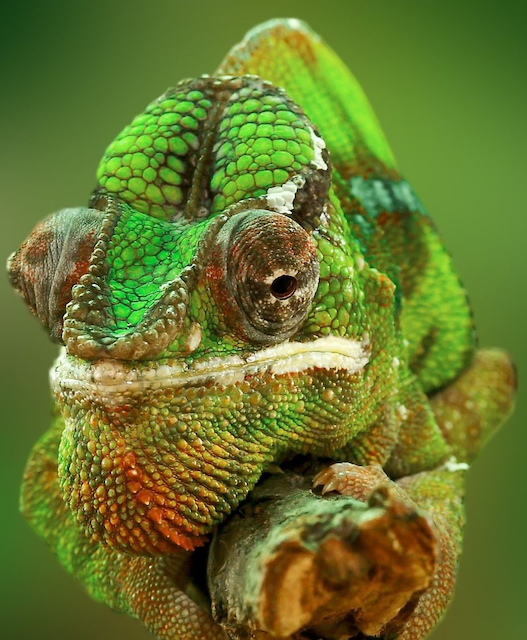
\includegraphics[height=6cm]{figures/chamaeleon_hochformat}

				{\tiny \textcolor{digiPH_darkorange}{Bildquelle: \url{pixabay.com}, CC-0}}
			\end{center}
		\end{column}
		\begin{column}{5cm}
			\begin{center}
				\Large
				Bitte mit Bedacht!
			\end{center}
			\pause
			\begin{center}
				Nicht mehr als ein bis zwei verschiedene Schriftfarben verwenden (Ruhe, bessere Lesbarkeit).
			\end{center}
			\begin{center}
				Tipp: Lieber durch Bilder Abwechslung schaffen!
			\end{center}
		\end{column}
	\end{columns}
\end{frame}

\begin{frame}
	%Gambar besar dengan penjelasan tanpa judul
	\begin{center}
		
\includegraphics[height=6cm]{figures/kopfhoerer}

		{\tiny \textcolor{digiPH_darkorange}{Nicht die Bildquelle und die Lizenz vergessen! Bildquelle: \url{pixabay.com}, CC-0}}
	\end{center}
	\begin{center}
		Haben Sie Mut zur Vereinfachung und zu ungewohnter Positionierung und finden Sie interessante Ausschnitte.
	\end{center}
\end{frame}

\begin{frame}{Gambar besar dengan judul dan penjelasan}
	\begin{center}
		
\includegraphics[height=5.5cm]{figures/placeholder}

		{\tiny \textcolor{digiPH_darkorange}{Bildquelle: \url{pixabay.com}, CC-0}}
	\end{center}
	\begin{center}
		Geschlechtsneutrales Formulieren ist uns wichtig: bei unseren eLectures ebenso. \textbf{In Schrift, Wort und Bild!}
	\end{center}
\end{frame}


\begin{frame}{Gambar dengan penjelasan sebelumnya}
	\small Ihre eLecture wird zum Nachsehen aufgezeichnet und veröffentlicht. Deshalb muss sie inhaltlich und urheberrechtlich korrekt sein!

	\tiny Weiteres dazu entnehmen Sie bitte dem Infoblatt: \url{http://www.virtuelle-ph.at/selbst-electures-abhalten/infoblatt}

	\small Die Teilnehmenden werden über einen Disclaimer zu Beginn der eLecture darüber informiert:

	\begin{center}
		
\includegraphics[height=3.5cm]{figures/placeholder}

		{\tiny \textcolor{digiPH_darkorange}{Bildquelle: Lene Kieberl, \href{https://creativecommons.org/licenses/by/3.0/at/}{CC BY}}}
	\end{center}
\end{frame}

\begin{frame}[t]{Tiga Gambar}

\hfil\hfil
\includegraphics[width=5cm]{figures/placeholder}\newline
  \null\hfil\hfil\makebox[5cm]{Lorem}\newline
  \vfil
  \hfil\hfil{
\includegraphics[width=5cm]{figures/placeholder}}\hfil\hfil
    {
\includegraphics[width=5cm]{figures/placeholder}}\newline
  \null\hfil\hfil{\makebox[5cm]{Lorem}}
    \hfil\hfil{\makebox[5cm]{Lorem}}

\end{frame}

\begin{frame}{Kolom dengan foto orang}
	\begin{columns}
		\begin{column}{5cm}
			\small besonders aber bei Minderjährigen bitte unbedingt abklären, ob diese bzw. ihre Erziehungsberechtigten mit der Veröffentlichung einverstanden sind (Recht am eigenen Bild).
		\end{column}
		\begin{column}{5cm}
			\begin{center}
				
\includegraphics[height=2.5cm]{figures/placeholder}

				{\tiny \textcolor{digiPH_darkorange}{Bildquelle: Details Foto XY, \url{pixabay.com}, CC-0}}
			\end{center}
		\end{column}
	\end{columns}
	\begin{columns}
		\begin{column}{5cm}
			\begin{center}
				
\includegraphics[width=5cm]{figures/placeholder}

				{\tiny \textcolor{digiPH_darkorange}{Bildquelle: Details Foto XY, \url{pixabay.com}, CC-0}}
			\end{center}
		\end{column}
		\begin{column}{5cm}
			\begin{block}{\small Tipp:}
				\scriptsize
				Als Hilfestellung können Sie vielleicht unseren \enquote{Schummelzettel OER} mit Tipps und Quellen für verwendbare Bilder nutzen, den Sie hier zum Download vorfinden:\\
				\url{http://www.virtuelle-ph.at/schummelzettel}
			\end{block}
		\end{column}
	\end{columns}
\end{frame}

\begin{frame}{Sie möchten Software/Seiten live vorzeigen?}
	% Schriftgröße verkleinern
	\scriptsize
	% Absatzabstand einstellen
	\setlength{\parskip}{0.75\baselineskip}

	Beachten Sie bitte, dass Sie beim Zeigen von längeren Ausschnitten einer \textbf{Programmoberfläche} (Vorzeigen von Abläufen die nicht mehr durch das Zitatrecht abgedeckt sind) gegebenenfalls die \textbf{Erlaubnis der Herstellerfirma einholen müssen}, sofern Sie nicht Urheber/in sind bzw. keine lizenzrechtliche Erlaubnis zur Vorführung vorliegt (mehr Info: \url{http://bit.ly/vphuhr}).

	\textbf{Diese Angabe kann Ihre Co-Moderation für Sie einblenden, bitte teilen Sie sie bei Testtermin oder via Email mit.}

	\begin{block}{\scriptsize Beispiel: Live-Demo \href{GIMP}{http://www.gimp.org/},GNU General Public License 29.01.2018}
		\centering
		
\includegraphics[height=4cm]{figures/placeholder}
	\end{block}
\end{frame}

%\end{comment}
%\begin{comment}

% Hanya untuk Navigasi Miniframe
\miniframesoff
\begin{frame}<beamer>{}
	\begin{center}
		\ldots Manege frei für Ihr Knowhow und Ihre Folien!
	\end{center}
	\vspace{3cm}
	\tiny
	PS: Am Ende Ihrer eLecture weist Ihre Co-Moderation die Teilnehmenden noch auf weitere Angebote (\zB der aktuellen Online-Tagung) und die Social-Media-Präsenzen hin. Wir bitten Sie auch um Weiterverbreitung unseres (und Ihres!) Lernangebots. Selbst schon geliked? Wir freuen uns über Likes, Kommentare und natürlich Follower!
\end{frame}
%\end{comment}

%\begin{frame}{\enquote{Stopfen} Gambar dengan qoute digambar \ldots}
%	\framesubtitle{Arbeiten Sie mit Bildern: online lieber mehrere, weniger dichte Folien zeigen!}
%	\begin{center}
%		\begin{tikzpicture}
%			\node[anchor=south west,inner sep=0] (bild) at (0,0) {
\includegraphics[width=0.88\textwidth]{figures/placeholder}};
%			\begin{scope}[x=(bild.south east),y=(bild.north west)]
%				% Gitternetz einzeichnen
%				%\draw[help lines] (0,0) grid[xstep=0.1,ystep=0.1] (1,1);
%				% Text einfügen
%				\node[font=\scriptsize,align=left,color=white,text width=4cm] (text) at (0.79,0.3) {Bitte verwenden Sie ausschließlich urheberrechts-einwandfreies Bildmaterial (NoGo: Schulbücher!)\\
%				Am besten also: eigenes und/oder CC-Bildmaterial, \zB von \url{www.pixabay.com} oder ähnlichen Plattformen!\\
%				Bitte nie eine sichtbare Bildquelle und Lizenz vergessen.};
%			\end{scope}
%		\end{tikzpicture}
%
%		{\tiny \textcolor{digiPH_darkorange}{Bildquelle: David Bogner, 2015, \href{https://creativecommons.org/licenses/by-nc-sa/3.0/at/}{CC BY-NC-SA}}}
%	\end{center}
%\end{frame}

\begin{frame}<beamer>{}
\bibliographystyle{apalike}
{\tiny
\bibliography{biblio.bib}
}
\end{frame}

\end{document}
